\documentclass[11pt]{article}

\usepackage[margin=1in]{geometry}
\usepackage{amsmath,amssymb,amsthm}
\usepackage{mathtools}
\usepackage{booktabs}
\usepackage{graphicx}
\usepackage{hyperref}
\usepackage{xcolor}
\usepackage{enumitem}
\usepackage{titlesec}
\usepackage{fancyhdr}

\hypersetup{colorlinks=true, linkcolor=blue!50!black, citecolor=blue!50!black,
            urlcolor=blue!50!black}
\titleformat{\section}{\large\bfseries}{\thesection}{0.6em}{}
\titleformat{\subsection}{\normalsize\bfseries}{\thesubsection}{0.6em}{}
\pagestyle{fancy}\fancyhf{}
\rhead{\small Avellaneda--Stoikov Quoting in Credit}\lhead{\small \thepage}

\theoremstyle{definition}
\newtheorem{definition}{Definition}
\newtheorem{remark}{Remark}
\theoremstyle{plain}
\newtheorem{proposition}{Proposition}
\newtheorem{theorem}{Theorem}

\newcommand{\E}{\mathbb{E}}
\newcommand{\dd}{\mathrm{d}}

\title{\textbf{Avellaneda--Stoikov Optimal Quoting,\\ Adapted to Credit Spreads}\\[4pt]
\large A Synthetic-Data Study of Inventory-Aware Dealer Behaviour}
\author{\textit{ascredit} project documentation}
\date{\today}

\begin{document}
\maketitle

\begin{abstract}
\noindent
We recast the Avellaneda--Stoikov (AS) optimal market-making model from price
space into \emph{credit-spread} space and study the resulting dealer policy by
Monte Carlo simulation over synthetic spread paths and a reduced-form Poisson
order flow. Three adaptations are required: the credit spread becomes the state
variable; inventory risk is scaled by spread duration (DV01); and the quote
skew acquires the opposite sign, because price moves inversely to spread.
We give the closed-form reservation spread and optimal quotes, derive the
distribution of the dealer's profit and loss (P\&L), and show numerically that
the inventory-aware policy trades a small amount of expected edge for a large
reduction in inventory and P\&L variance. \textbf{All data are synthetic; this
is a study of optimal quoting behaviour, not a historical backtest, and not
investment advice.}
\end{abstract}

\tableofcontents
\bigskip

%======================================================================
\section{The market-making problem}
A dealer continuously posts a bid and an ask and earns the quoted half-spread
on each fill, while bearing the risk that the asset's value moves against the
inventory accumulated from one-sided flow. Avellaneda and Stoikov (2008) solve
this as a stochastic-control problem for a CARA dealer whose asset mid follows
arithmetic Brownian motion, yielding closed-form approximations for the
\emph{reservation price} and the optimal bid/ask quotes.

%======================================================================
\section{From price space to spread space}
\label{sec:credit}

\begin{definition}[State variable]
For a corporate credit instrument the natural risk driver is the mid credit
spread $s_t$ (in basis points), not a price. We model it as a positivity-floored
mean-reverting diffusion,
\begin{equation}
\dd s_t=\kappa(\theta-s_t)\,\dd t+\sigma\,\dd W_t,\qquad s_t\ge s_{\min}>0,
\label{eq:ou}
\end{equation}
recovering the AS arithmetic-Brownian baseline when $\kappa=0$.
\end{definition}

\begin{definition}[DV01-scaled risk]
Dealer P\&L is a \emph{price} quantity, and price is locally linear in spread
through (minus) the spread duration, or DV01. A spread change $\dd s$ maps to a
price change $-\text{DV01}\cdot \dd s$ per unit face. Hence the volatility that
enters the control problem is the \emph{price} volatility
$\sigma_{\text{eff}}=\text{DV01}\cdot\sigma$, and inventory $q$ is measured in
DV01 (risk-equivalent) units.
\end{definition}

%======================================================================
\section{Reservation spread and optimal quotes}
\label{sec:quotes}

Let $q$ be signed inventory in DV01 units ($q>0$ = long credit risk),
$\gamma>0$ the risk aversion, $T$ the session horizon, and fill intensity
$\lambda(\delta)=A\,e^{-k\delta}$ at quoted distance $\delta$ from mid.

\begin{proposition}[Reservation spread]
The indifference (reservation) spread is
\begin{equation}
r(s,q,t)=s+q\,\gamma\,\sigma_{\text{eff}}^2\,(T-t).
\label{eq:res}
\end{equation}
\end{proposition}

\begin{proposition}[Optimal total width and quotes]
The optimal total quoted width is
\begin{equation}
\delta_{\text{tot}}(t)=\gamma\,\sigma_{\text{eff}}^2\,(T-t)
+\tfrac{2}{\gamma}\ln\!\big(1+\tfrac{\gamma}{k}\big),
\label{eq:width}
\end{equation}
and the dealer posts, in spread space,
\begin{equation}
\text{bid}=r+\tfrac{\delta_{\text{tot}}}{2}\ \ (\text{client sells bond}),
\qquad
\text{ask}=r-\tfrac{\delta_{\text{tot}}}{2}\ \ (\text{client buys bond}).
\label{eq:quotes}
\end{equation}
\end{proposition}

\begin{remark}[The sign of the skew --- a bug we hit]
\label{rem:sign}
In price space a long-inventory dealer shades the reservation price \emph{down}
to attract buyers. In spread space price is \emph{inverse} to spread, so a
long-credit dealer must shade the reservation spread \emph{up}: by
(\ref{eq:res}) with $q>0$, $r>s$, which widens the bid distance (fewer trades
that lengthen the book) and tightens the ask distance (more trades that flatten
it). Implementing the price-space sign here makes the policy \emph{accumulate}
risk instead of shedding it. The regression test
\texttt{test\_as\_controls\_inventory\_better\_than\_symmetric} guards against
exactly this inversion.
\end{remark}

%======================================================================
\section{P\&L accounting}
On each fill the dealer captures edge $|\,\text{quote}-s\,|\cdot\text{DV01}$ per
clip; inventory marks to market at $-q\,\text{DV01}\,\dd s$ (a long-credit book
loses when spreads widen). Total session P\&L is the sum of realised capture and
running inventory mark.

%======================================================================
\section{Simulation results}
\label{sec:results}

Over $4{,}000$ synthetic sessions at an illustrative investment-grade
calibration, the inventory-aware (AS) policy is compared to an
inventory-agnostic symmetric benchmark.

\begin{table}[h]\centering\small
\begin{tabular}{@{}lrr@{}}
\toprule
 & \textbf{AS} & \textbf{Symmetric}\\
\midrule
mean P\&L & 423.8 & 432.5\\
P\&L std & \textbf{40.6} & 47.0\\
risk-adjusted ratio & \textbf{10.45} & 9.20\\
std of terminal inventory & \textbf{4.54} & 9.89\\
\bottomrule
\end{tabular}
\caption{Baseline calibration, 4{,}000 sessions (synthetic).}
\end{table}

\noindent
The AS policy gives up a little expected edge for a large reduction in both
inventory dispersion and P\&L variance --- the signature AS trade-off.

\begin{figure}[h]\centering
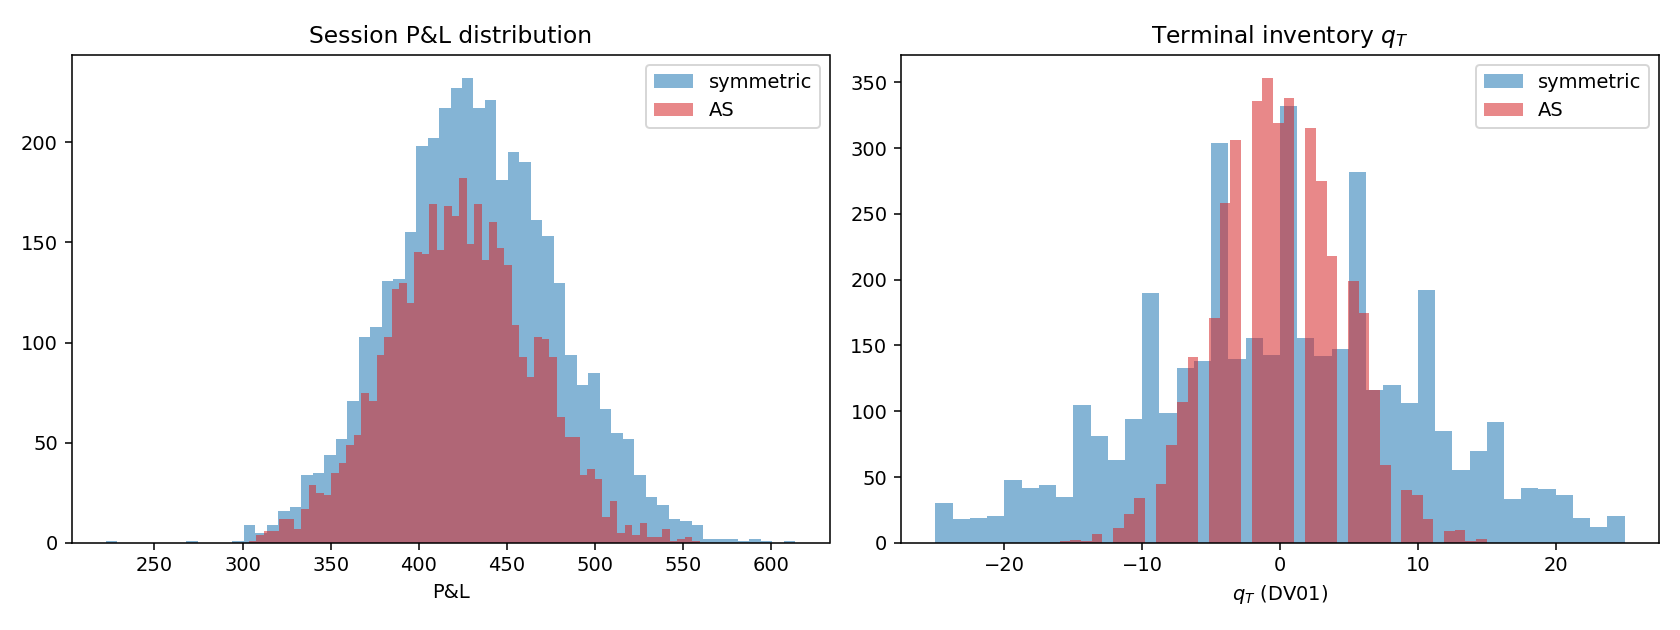
\includegraphics[width=0.75\linewidth]{../figures/montecarlo.png}
\caption{Session P\&L and terminal-inventory distributions, AS vs symmetric.}
\end{figure}

\begin{figure}[h]\centering
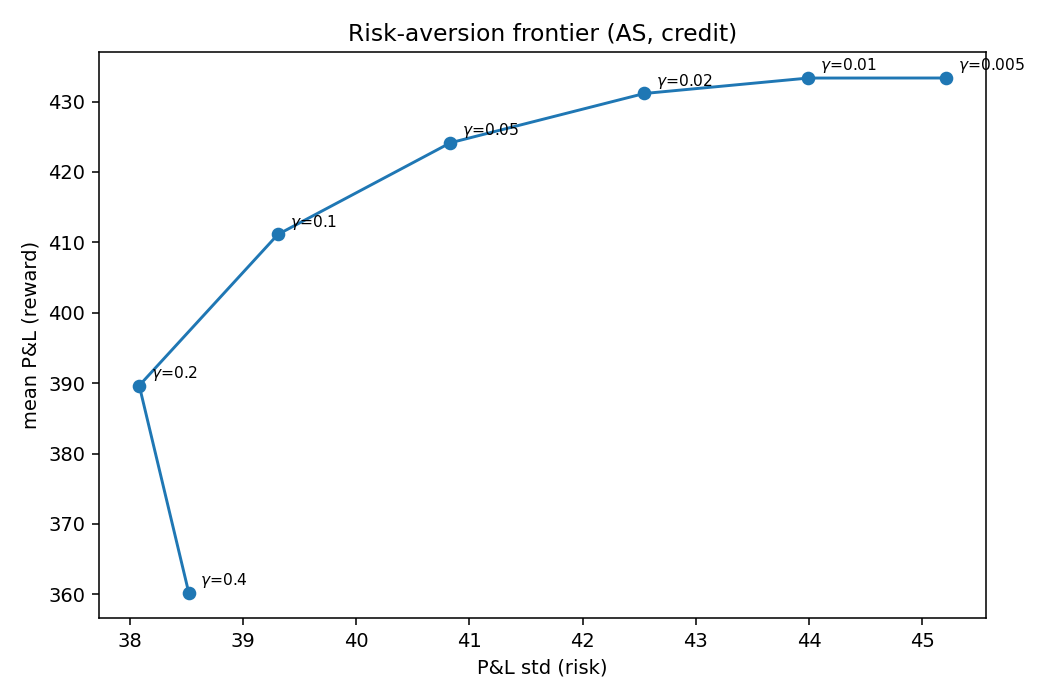
\includegraphics[width=0.62\linewidth]{../figures/frontier.png}
\caption{Risk-aversion frontier: mean P\&L vs P\&L std as $\gamma$ varies.}
\end{figure}

%======================================================================
\section{Limitations and extensions}
\label{sec:limits}
The model uses reduced-form Poisson flow (no adverse selection), treats bonds as
independent (no portfolio inventory penalty or spread correlation), uses a
first-order DV01 P\&L (no convexity or jump-to-default), and ignores funding,
hedging and transaction costs. Each is a natural extension; none changes the
qualitative inventory-control result.

\section*{Reference}
\addcontentsline{toc}{section}{Reference}
\small
Avellaneda, M. \& Stoikov, S. (2008). High-frequency trading in a limit order
book. \emph{Quantitative Finance}, 8(3), 217--224.

\vfill
\noindent\rule{\linewidth}{0.4pt}\\
{\footnotesize\textbf{Disclaimer.} All spread paths, order flow and P\&L are
synthetic. This document is educational and is not investment, financial, or
trading advice.}

\end{document}
